\documentclass[UserManual.tex]{subfiles}
\begin{document}
\setcounter{section}{10}

\section{Underlying Theory of {\it Smooth Emulator}}\label{sec:theory}

A detailed explanation of the underlying theory used by {\it Smooth Emulator} and {\it Smooth Training Point Optimizer} is provided in the accompanying paper \href{./smoothdraft.pdf}{{\tt smoothdraft.pdf}}, which can be found in the same directory as this paper.

The choice of model emulators, $E(\vec{\theta})$, depends on the prior understanding of the model being emulated, $M(\vec{\theta})$, which we refer to as the ``full model''. If one knows that  a function is linear, then a linear fit is clearly the best choice. Whereas to reproduce lumpy features with a single scale, where the lumps have a characteristic length scale, Gaussian process emulators are highly effective, but may require large training sets to resolve the peaks. The quality of an emulator can be assessed through the following criteria:
\begin{itemize}
  \item $E(\vec{\theta}_t)=M(\vec{\theta}_t)$ at the training points, $\vec{\theta}_t$. 
  \item The emulator should reasonably reproduce the model away from the training points. This should hold true for either interpolation or extrapolation.
  \item The emulator should reasonably represent its uncertainty
  \item A minimal number of training points should be needed
  \item The method should easily adjust to larger numbers of parameters, $\theta_i,~i=1\cdots N$
  \item The emulator should not be affected by rotations or translations of the parameter space
  \item The emulator should be able to account for noisy models (at which point the prediction would not necessarily exactly reproduce the training data)
  \item Training and running the emulator should not be numerically intensive
\end{itemize}
Here the goal is to focus on a particular class of functions: functions that are {\it smooth}. Smoothness is a prior knowledge of the function. It is an expectation that the linear terms of the function are likely to provide more variance than the quadratic contributions, which are in turn likely to be more important than the cubic corrections, and so on. 

\subsection{Mathematical Form of {\it Smooth Emulator}}

To satisfy the criteria above, the functional form of the emulator in $N_{\rm pars}$ dimensional parameter space, $\theta_1\cdots\theta_N$, is
\begin{eqnarray}
Y(\vec{\theta})&=&e^{-|\vec{\theta}|^2/2\Lambda^2}
\sum_{\vec{n}} \frac{A_{\vec{n}}}{\sqrt{n_1!\cdots n_N!}}\left(\frac{\theta_1}{\Lambda}\right)^{n_1}\cdots\left(\frac{\theta_1}{\Lambda}\right)^{n_N},
\end{eqnarray}
where the assumed-to-be-independent coefficients $A_{\vec{n}}$ are assumed to have a Gaussian distributions,
\begin{eqnarray}\label{eq:Aprior}
P(A_n)&=& \frac{1}{(2\pi\sigma_A^2)^{1/2}}e^{-A_n^2/2\sigma_A^2}.
\end{eqnarray}
Here, $\Lambda$ and $\sigma_A$ are what is known as hyper-parameters, i.e. they are not parameters of the full-model, but are parameters that define the emulator. The hyper-parameter $\Lambda$ will be referred to as the convergence parameter and defines the expected relative strengths of various orders in the Taylor expansion. The hyper-parameter $\sigma_A$ describes the characteristic strength of the coefficients. The coefficients $\vec{A}_{\vec{n}}$ are not referred to as hyper-parameters, but in practice the hyper-parameters $\vec{A}_{\vec{n}}$, $\sigma_A$ and $\Lambda$ are all treated similarly, in that they are all required to define the training data, and they are all allowed to vary according to some prior. Whereas the prior for the coefficients $A_{\vec{n}}$ is defined in Eq. (\ref{eq:Aprior}), the priors for $\sigma_A$ and $\Lambda$ are generally assumed to be flat, though that can be changed. For example, one might simply state that $\Lambda$ is constrained to be within some window, or might even be fixed.

With this from the correlation between two points is
\begin{eqnarray}
\langle Y(\vec{\theta}_1)Y(\vec{\theta}_2)\langle &=& \sigma_A^2 C_0(\vec{\theta}_1,\vec{\theta}_2),\\
\nonumber
C_0(\vec{\theta}_1,\vec{\theta}_2)&=&e^{-|\vec{\theta}_1-\vec{\theta}_2|^2/2\Lambda^2},
\end{eqnarray}
where the averaging refers to an average over the coefficients $A_{\vec{n}}$. Rather than averaging over the coefficients, one could maximize the likelihood, but the resulting expression is identical. One can find the most likely set of coefficients that reproduces the values of the full model runs for a given $\sigma_A$ and $\Lambda$. This leads to an optimized prediction
\begin{eqnarray}\label{eq:Yemu}
Y_{\rm opt}(\vec{\theta})&=&\sum_{ab}C_0(\vec{\theta},\vec{\theta}_a)B^{-1}_{ab}y_b,\\
\label{eq:Bdef}
B_{ab}&=&C_0(\vec{\theta}_a,\vec{\theta}_b)+\alpha^2\delta_{ab}.
\end{eqnarray}
Here, $y_a$ are the values of the full model calculations measured at the training point $\vec{\theta}_a$, and $\alpha$ is a measure of the point-by-point noise. If one thinks that the calculated values vary randomly by one percent of the characteristic values, one would set $\alpha=0.01$. Remarkably, this is exactly the same expression as for a Gaussian process (GP) emulator with a quadratic kernel. This derives from the fact that any two distributions with the same correlation result in the same emulator, a.k.a the `kernel trick'.  The emulator prediction in Eq. (\ref{eq:Yemu}) is independent of $\sigma_a$, but depends on $\Lambda$. 

The emulator's uncertainty (for fixed $\sigma_A$ and $\Lambda$) is:
\begin{eqnarray}
\langle \delta Y(\vec{\theta})^2\rangle&=&
\sigma_A^2\left[1-\sum_{ab}C_0(\vec{\theta},\vec{\theta}_a)B^{-1}_{ab}C_1(\vec{\theta}_b,\vec{\theta})\right].
\end{eqnarray}
This expression assumes fixed $\sigma_A$ and $\Lambda$. This expression ignores the contribution from the uncertainties in the hyper-parameters. Including those uncertainties is described below.

The likelihood distributions for $\sigma_A$ and $\Lambda$ are given by the function
\begin{eqnarray}
Z(\sigma_A,\Lambda)&=&\int\prod_{\vec{i}}~P(\vec{A},\sigma_A,\Lambda)\\
\nonumber
&=&\sigma_A^{-N}(\det{B})^{-1/2}\exp\left[-\frac{1}{2\sigma_A^2}y_aB^{-1}_{ab}y_b\right],
\end{eqnarray}
where $P(\vec{A},\sigma_A,\Lambda)$ is the prior probability constrained by the training points. To calculate the uncertainties, {\it Smooth Emulator} uses the maximum likelihood values of $\sigma_A$ and $\Lambda$, but when including the additional emulator uncertainty due to the fact that $\sigma_A$ and $\Lambda$ vary, {\it Smooth Emulator} uses the curvature of $Z(\sigma_A,\Lambda)$.
The uncertainty for the emulator is then
\begin{eqnarray}\label{eq:delY2}
\langle\delta Y(\vec{\theta})^2\rangle&=&
\nonumber
\sigma_A^2\left[1-\sum_{ab}C_0(\vec{\theta},\vec{\theta}_a)B^{-1}_{ab}C_0(\vec{\theta}_b,\vec{\theta})\right]\\
\nonumber
&&+W_{\sigma_A\sigma_A}\left(\frac{\partial Y}{\partial\sigma_A}\right)^2
+2W_{\sigma_A\Lambda}\left(\frac{\partial Y}{\partial\sigma_A}\right)\left(\frac{\partial Y}{\partial\Lambda}\right)
%\nonumber
+W_{\Lambda\Lambda}\left(\frac{\partial Y}{\partial\Lambda}\right)^2.
\end{eqnarray}
Here, $W_{\alpha\beta}$ are the derivatives of $\ln(Z)$. All derivatives are calculated at the point of maximum likelihood. One can find a detailed explanation of these expressions in \href{./smoothdraft.pdf}{{\tt smoothdraft.pdf}}, including analytic expressions for $W$ and for $\partial Y/\partial\alpha$.

From here on, the function $Y(\vec{\theta})$ and the uncertainties will refer to expressions where the coefficients $A_{\vec{n}}$ are chosen to optimize the likelihood for a given $\sigma_A$ and $\Lambda$ and where $\sigma_A$ and $\Lambda$ were chosen to optimize $Z(\sigma_A,\Lambda)$.

\subsection{Training-Point Optimization}

Training-point locations should be chosen to minimize the uncertainty defined in Eq. (\ref{eq:delY2}) integrated over the prior. If the hyper-parameters are labeled by some vector $\vec{h}$, one would like to minimize
\begin{eqnarray}\label{eq:delY2bar}
\langle\langle \delta Y^2\rangle\rangle&=&
\int d\vec{h}~P(\vec{h})\langle \delta Y^2\rangle(\vec{h}).
\end{eqnarray}
However, one must choose training points (at least the first set) before one has actually run the full model. The last several terms in Eq. (\ref{eq:delY2}) depend on the values of the full model at the training points, $y_a$, or more precisely on the matrix $y_ay_b$. This can be replaced by the prior expectation, $y_ay_b\rightarrow \sigma_A^2C_0(\vec{\theta}_a,\vec{\theta}_b)$. The resulting estimate in Eq. (\ref{eq:delY2bar}) is the product of $\sigma_A^2$ multiplied by a complicated function of $\Lambda$ and the locations of the training points. One does not know, a priori, either $\sigma_A$ or $\Lambda$. Fortunately the value of $\sigma_A^2$ is irrelevant in determining the optimized positions. However, the optimized positions does depend on the value of $\Lambda$. Thus, in choosing the training points, one needs to first choose a value for $\Lambda$. Fortunately, from some studies, the choice of best positions is not strongly sensitive to $\Lambda$, i.e. if one chooses $\Lambda=2.5$ or $\Lambda=3$, the resulting positions vary rather little. 

Once one has chosen a reasonable value for $\Lambda$ one can fortunately find analytic expressions for $\langle\langle \delta Y^2\rangle\rangle/\sigma_A^2$. The expressions, which are provided in \href{./smoothdraft.pdf}{{\tt smoothdraft.pdf}}, are rather messy, so finding the optimized points involves a search through all possible $N_{\rm pars}$ dimensional positions of $N_{\rm train}$ points. In {\it Smooth Emulator} this is accomplished by a simple steepest decent algorithm. The procedure takes little time when $N_{\rm pars}\lesssim$ a dozen, but can begin to require minutes or even a few hours for $N_{\rm pars}\gtrsim$ two dozen. 

Figure \ref{fig:Sigma2vsNpars} shows the expected accuracy as a function of the number of model parameters. Even if the number of training points rises quadratically with the number of parameters (as shown in the figure), the expected accuracy rises substantially with $N_{\rm pars}$. A detailed discussion of the pernicious nature of higher dimensions can be found in  \href{./smoothdraft.pdf}{{\tt smoothdraft.pdf}}. The accuracy strongly improves for higher convergence parameters, $\Lambda$, as shown in Fig. \ref{fig:Sigma2vsLambda}. More training points leads to better accuracy, as shown in Fig. \ref{fig:Sigma2vsNTrain}. The expected uncertainty shown in Fig. \ref{fig:Sigma2vsNTrain} has noticeable kinks in the behavior. The number of parameters at which these kinks occur correspond to the number of parameters required for linear, quadratic, cubic fits $\cdots$. For linear fits, that number is $N_{\rm pars}+1$, for quadratic it is $(N_{\rm pars}+1)(N_{\rm pars}+2)/2$ and for cubic fits, $(N_{\rm pars}+1)(N_{\rm pars}+2)(N_{\rm pars}+3)/6$. Given the kinks, it might behoove the User to choose a number of traininig points corresponding to the locations of these kinks. Finally, Fig. \ref{fig:Sigma2vsNsteps} shows the expected accuracy as a function of the number of steps in the steepest descent algorithm. Because the algorithms can start with either a random placement of trainiig points, or with a selection using a Latin hyper-cube algorithm, one can see the expected benefit of this optimization procedure relative to simply choosing the points randomly or using Latin hyper-cube sampling. Typically the improvement is on the order of a factor of two, with larger relative improvements for more parameters or more training points. This improvement can also be expressed by stating how many fewer training points one would need to consider to achieve the same accuracy. Roughly, this might be approximately a third fewer points for most cases.

In {\it Smooth Emulator} the optimization procedure first reads the file describing the prior model-parameter distribution. The prior distributions is assumed to an independent product of priors for each model parameter. Each distribution is assumed to be either a Gaussian, defined by a location and width, or a uniform distribution within some minimum and maximum values. {\it Smooth Emulator} scales all the model parameters to variables centered at the origin and with variances of three. I.e., the scaled model-parameters have prior distributions that are either proportional to $e^{-3\theta_i^2/2}$ or uniform within the range $-1<\theta_i<1$. If one expected variation of the observable to be similar with respect to changing any of these variables, it would make sense to apply a single value of $\Lambda$ for all $N_{\rm pars}$ model parameters.

Given the strong dependence on the number of parameters and on $\Lambda$ the User might wish to consider higher values of $\Lambda$ for those model parameters expected to result in less variation of the observables within the prior. In {\it Smooth Emulator} this is accomplished by changing the widths of the priors, rather than assigning different values of $\Lambda$. One chooses a single value of $\Lambda$ to represent the convergence of the most sensitive model parameters. One then reduces the widths of the priors for the less important model parameters. Each model parameter is assigned a sensitivity, $s_i$. The priors for Gaussian and uniform distributions are then set to $e^{-3\theta_i^2/2s_i^2}$ or to $s_i<\theta_i<s_i$. In practice, this is identical to assigning different values of $\Lambda$ to each parameter scaled as $1/s_i$. This can be especially if there are large numbers of weakly sensitive parameters. For example, if one had 20 model parameters where the appropriate value of $\Lambda$ was 2.5 for 5 parameters, but the appropriate value for the majority was closer to 4, one would set $\Lambda=2.5$, then set $s_i=1$ for the handful of more important parameters, and set $s_i=5/8$ for the others. The optimization procedure would select training points to best capture the variation due to the first five parameters and worry less about positioning the points to capture higher-order polynomial behavior in the other parameters. The final estimate of the emulator's uncertainty would also be significantly reduced.

\begin{figure}
\begin{minipage}{0.475\textwidth}
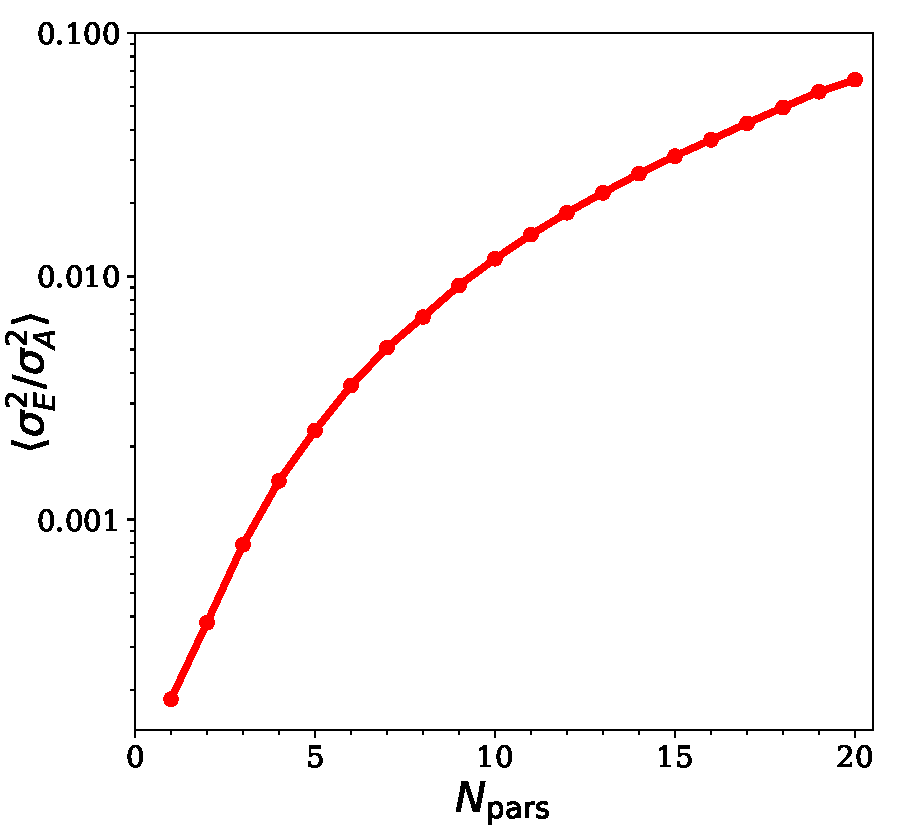
\includegraphics[width=0.95\textwidth]{figs/sigma2vsNpars}
\caption{\label{fig:Sigma2vsNpars}
The accuracy metric as a function of the number of model parameters assuming Gaussian priors. The convergence parameter was set to $\Lambda=3$, the point-by-point noise was set to $\alpha=0.01$ and the number of training points was set to match the number of expansion coefficient of quadratic order or less. This illustrates the difficulty to accurately emulate higher dimensional functions even if the number of training points increases as $N_{\rm train}=(N_{\rm pars}+1)(N_{\rm pars}+2)/2$.}
\end{minipage}
\hspace*{0.025\textwidth}
\begin{minipage}{0.475\textwidth}
\includegraphics[width=\textwidth]{figs/Sigma2vsLambda}
\caption{\label{fig:Sigma2vsLambda}
The expected accuracy of the emulator falls rapidly with the convergence parameter $\Lambda$. For this illustration $N_{\rm pars}=6$ and the number of training points was set to 28, the number of expansion coefficients of order $n=2$ or less. Calculations were repeated for different values of the point-by-point noise, $\alpha$. As expected, the impact of the point-by-point noise sets in as the accuracy of the emulator improves.}
\end{minipage}
\end{figure}

\begin{figure}
\begin{minipage}{0.475\textwidth}
\includegraphics[width=0.95\textwidth]{figs/sigma2vsNTrain_log}
\caption{\label{fig:Sigma2vsNTrain}
For all Gaussian priors, with $N_{\rm pars}=6$, $\Lambda=3$, and $\alpha=0.01$, the expected mean accuracy falls with increasing the number of training points. The minimum number of training points required for linear, quadratic and cubic fits are 7, 28 and 82. After passing one of these threhsolds the marginal improvement for additional training points decreases. For $N=8$, one can place the points in a simplex with an additional point at the center, and the symmetry of this configuration provides an especially large improvement. This behavior might inspire the modeler to choose a number of training points equal to one of the thresholds. The optimized placement significantly improves compared to Latin hyper-cube sampling.
}
\end{minipage}
\hspace*{0.025\textwidth}
\begin{minipage}{0.475\textwidth}
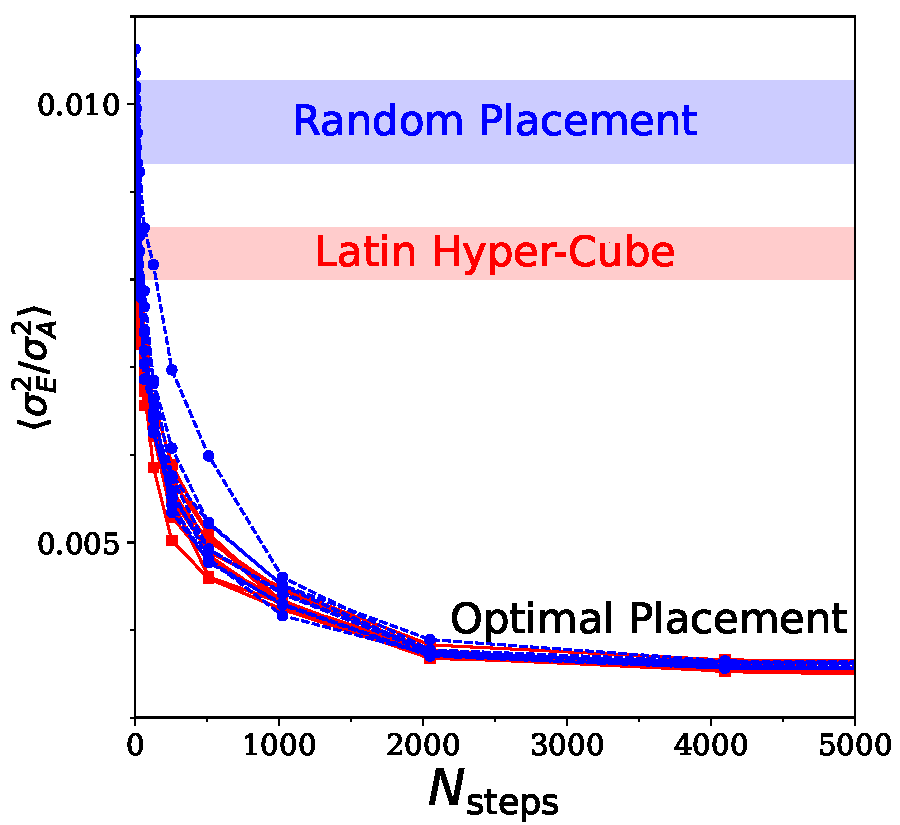
\includegraphics[width=\textwidth]{figs/sigma2vsNMC}
\caption{\label{fig:Sigma2vsNsteps}
The search procedure provides most of the improvement for the first few thousand steps. For this example, $N_{\rm pars}=6$, $\Lambda=3$ and $\alpha=0.01$ the number of training points was set to 28. Several initial configurations were considered. Those where the points were placed randomly (blue circles) tended to start at roughly three times the optimized value, whereas those that were initialized with Latin hyper-cube sampling tended to start at a bit less than double the optimized uncertainty. The bands roughly represent the spread of initial accuracies, and the fall from the bands to the optimal values represents the improvement one expects to gain through the optimization procedure.}
\end{minipage}
\end{figure}

\end{document}
